% ------------------------------------------------------------------------------
% 3.5. FLUJO OPERATIVO
% ------------------------------------------------------------------------------
\subsection{3.5. Flujo Operativo}\label{sec:flujo_operativo}

El flujo operativo describe cómo se desarrolla actualmente, en la Dirección Universitaria de Bienestar Social y Salud (DUBSS), el proceso de postulación y adjudicación de la Beca Comedor. En él intervienen el postulante, que presenta su carpeta con la documentación de respaldo; el personal de Trabajo Social, que revisa los documentos y califica la solicitud; y la Encargada de Sistemas, que incorpora el rendimiento académico y calcula el puntaje total que determina la adjudicación. La Figura~\ref{fig:postulacion_beca} representa las actividades de este proceso y las responsabilidades de cada actor.

\begin{figure}[H]
\caption{Diagrama de actividades del proceso de postulación a la Beca Comedor}
\label{fig:postulacion_beca}
\centering
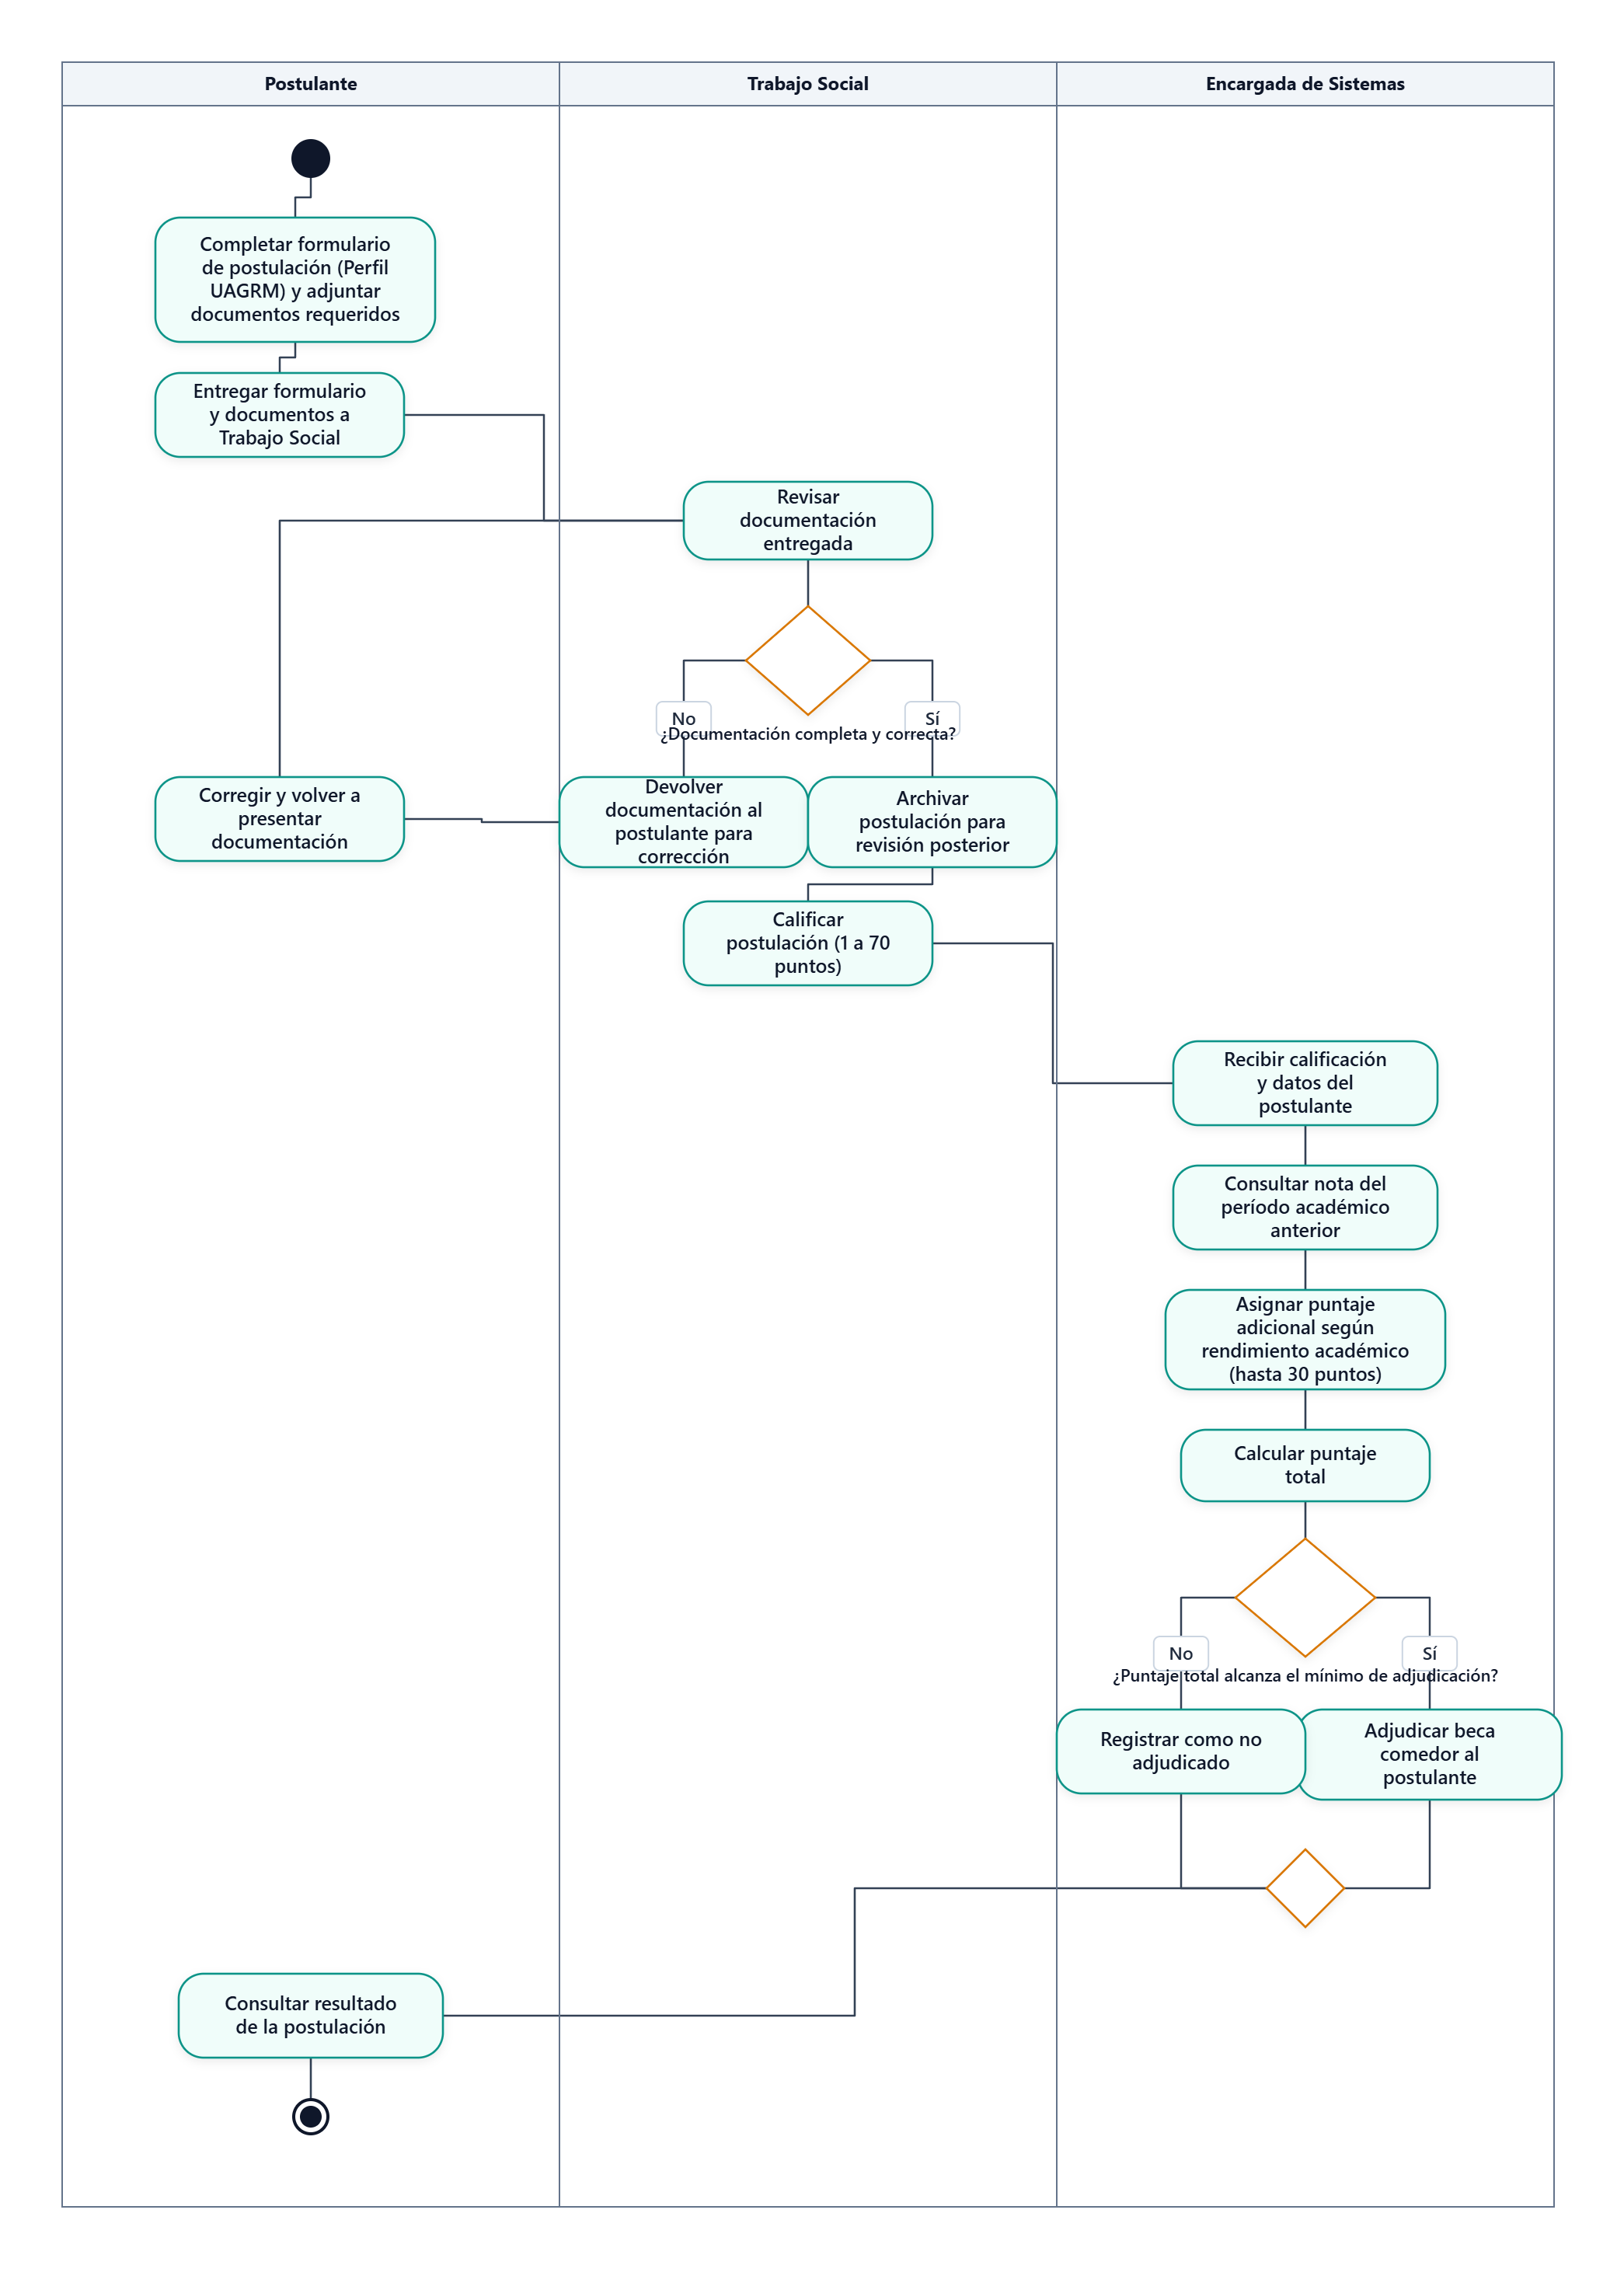
\includegraphics[width=\textwidth,height=0.8\textheight,keepaspectratio]{images/16_Postulacion_Beca.png}

\smallskip
\noindent\raggedright\textit{Nota.} Elaboración propia basado en la entrevista con el personal de la DUBSS.
\end{figure}
